
\documentclass[aspectratio=1610, 13pt]{beamer}
\usepackage{ctex}
\usepackage{CJKutf8}
\usepackage{xcolor}
\usepackage{multicol}
\usepackage{mathtools,array}
\usepackage[T1]{fontenc}
\usepackage{zi4}
\usepackage[font={scriptsize,bf}]{caption}
% \usepackage{subcaption}
\usepackage{graphics}
\usepackage{tikz}
\usepackage{fontawesome5}
\usepackage{mathpartir}

\newcommand{\naturals}{\mathbb{N}}
\newcommand{\reals}{\mathbb{R}}

\newcommand{\Dist}[1]{\mathcal{D}(#1)}
\newcommand{\expectation}{\mathbb{E}}

\newcommand{\states}{S}
\newcommand{\actions}{A}
\newcommand{\observables}{O}
\newcommand{\trans}{T}
\newcommand{\obs}{Z}
\newcommand{\reward}{R}
\newcommand{\discount}{\gamma}

\newcommand{\beliefs}{\mathcal{B}}
\newcommand{\beliefUpdate}{\tau}

\newcommand{\policy}{\pi}

\newcommand{\diff}[1]{\mathop{}\!\mathrm{d}#1}
\renewcommand{\figurename}{Figure}
\renewcommand{\refname}{Reference}

\AtBeginDocument{
  \catcode`_=12
  \begingroup\lccode`~=`_
  \lowercase{\endgroup\let~}\sb
  \mathcode`_="8000
}

% \usetheme{Madrid}
% % \usetheme{default}
% \setbeamertemplate{caption}[numbered]
% \setbeamerfont{title}{size=\large}
\mode<presentation>
{
  \usetheme{Darmstadt}      % or try Darmstadt, Madrid, Warsaw, ...
  \usecolortheme{default} % or try albatross, beaver, crane, ...
  \usefonttheme[onlymath]{serif}  % or try serif, structurebold, ...
  \setbeamertemplate{navigation symbols}{}
  \setbeamertemplate{caption}[numbered]
  \setbeamertemplate{footline}[frame number] 
} 

\usepackage{listings}
\lstdefinestyle{heaplang}{
    language=Caml,
    basicstyle=\footnotesize\ttfamily,
    keywordstyle=\color{blue},
    commentstyle=\color{red},
    escapeinside={<@}{@>},
    morekeywords={new_chan, fork, recv, send, swap, ref}
}
\lstdefinestyle{clang}{
    language=Caml,
    basicstyle=\footnotesize\ttfamily,
    keywordstyle=\color{blue},
    commentstyle=\color{red},
    escapeinside={<@}{@>},
}
\lstset{style=heaplang}

\usepackage{natbib}

\newcommand{\buchi}{B\"uchi }

\definecolor{goldenpoppy}{rgb}{0.99, 0.76, 0.0}
\definecolor{goldenyellow}{rgb}{1.0, 0.87, 0.0}
\definecolor{green2}{rgb}{0.1,0.7,0.3} 
\newcommand{\gcheck}{{\color{green2}\faCheckCircle[regular] }}
\newcommand{\rcross}{{\color{red} \faTimesCircle[regular]} }
\newcommand{\rflag}{{\color{red} \faFlag}}
% \usepackage{algorithm,amsmath}
% \usepackage[noend]{algpseudocode}

\newcommand{\zlstinline}{\let\par\endgraf\lstinline}
\newcommand{\comments}[1]{{\color{red}#1}}
\title{Group Meeting - 6}
\date{\today}
\author{Members: Yong Li, Depeng Liu, Weizhi Feng, Xie Li, Shizhen Yu, Yutian Zhu, Zongxin Liu}
\begin{document}
\maketitle
\begin{frame}\frametitle{内存安全工具开发}

进展情况:
\begin{itemize}
\item (刘宗鑫+李勰)利用SLAH API完成了从自己定义的分离逻辑公式到SLAH的分离逻辑公式的翻译模块,反馈了相关问题。
\item (李勰)对于一个基本块的符号执行进行了扩展,支持二元算术运算函数表达式的符号执行,目前正在实现\texttt{load}, \texttt{store}等函数表达式的符号执行。
\end{itemize}

存在问题:
\begin{itemize}
\item 不调用求解器的符号执行不精确的问题:对于\texttt{malloc},\texttt{free}以及指针算术导致的\texttt{blk}分裂。


\end{itemize}

目前的想法:
\begin{itemize}
\item 对指针算术的格式做一些约束,使得符号执行易于处理。(目前正在实现)
\end{itemize}

计划:
\begin{itemize}
\item 下周能有个单个Block从符号执行到验证走通的实现。
\item 硕士流程:开题。
\end{itemize}

\end{frame}

\begin{frame}{冯维直:Progress}
    \begin{itemize}
        \item 熟悉目前工具开发的Smack框架;
        \item 基于宗鑫写的Boogie CFG数据结构,实现了一个简单的lasso sampling(遇到分支以$1/2$概率选择后继),一次sample从原Boogie程序的CFG中得到一条路径,记录lasso的stem和loop;
          \item 实验Lasso
        Ranker支持的Boogie程序,尝试集成到我们的工具中(目前在尝试作为黑盒直接调用);
        \item 读LTL2BA文章,准备下周讲。
\end{itemize}    
\end{frame}

\begin{frame}{冯维直:Progress}
    \begin{itemize}
        \item 基于宗鑫写的Boogie CFG数据结构,实现了一个简单的lasso sampling(遇到分支以$1/2$概率选择后继),一次sample从原Boogie程序的CFG中得到一条路径,记录lasso的stem和loop;
            \begin{figure}[htbp]
    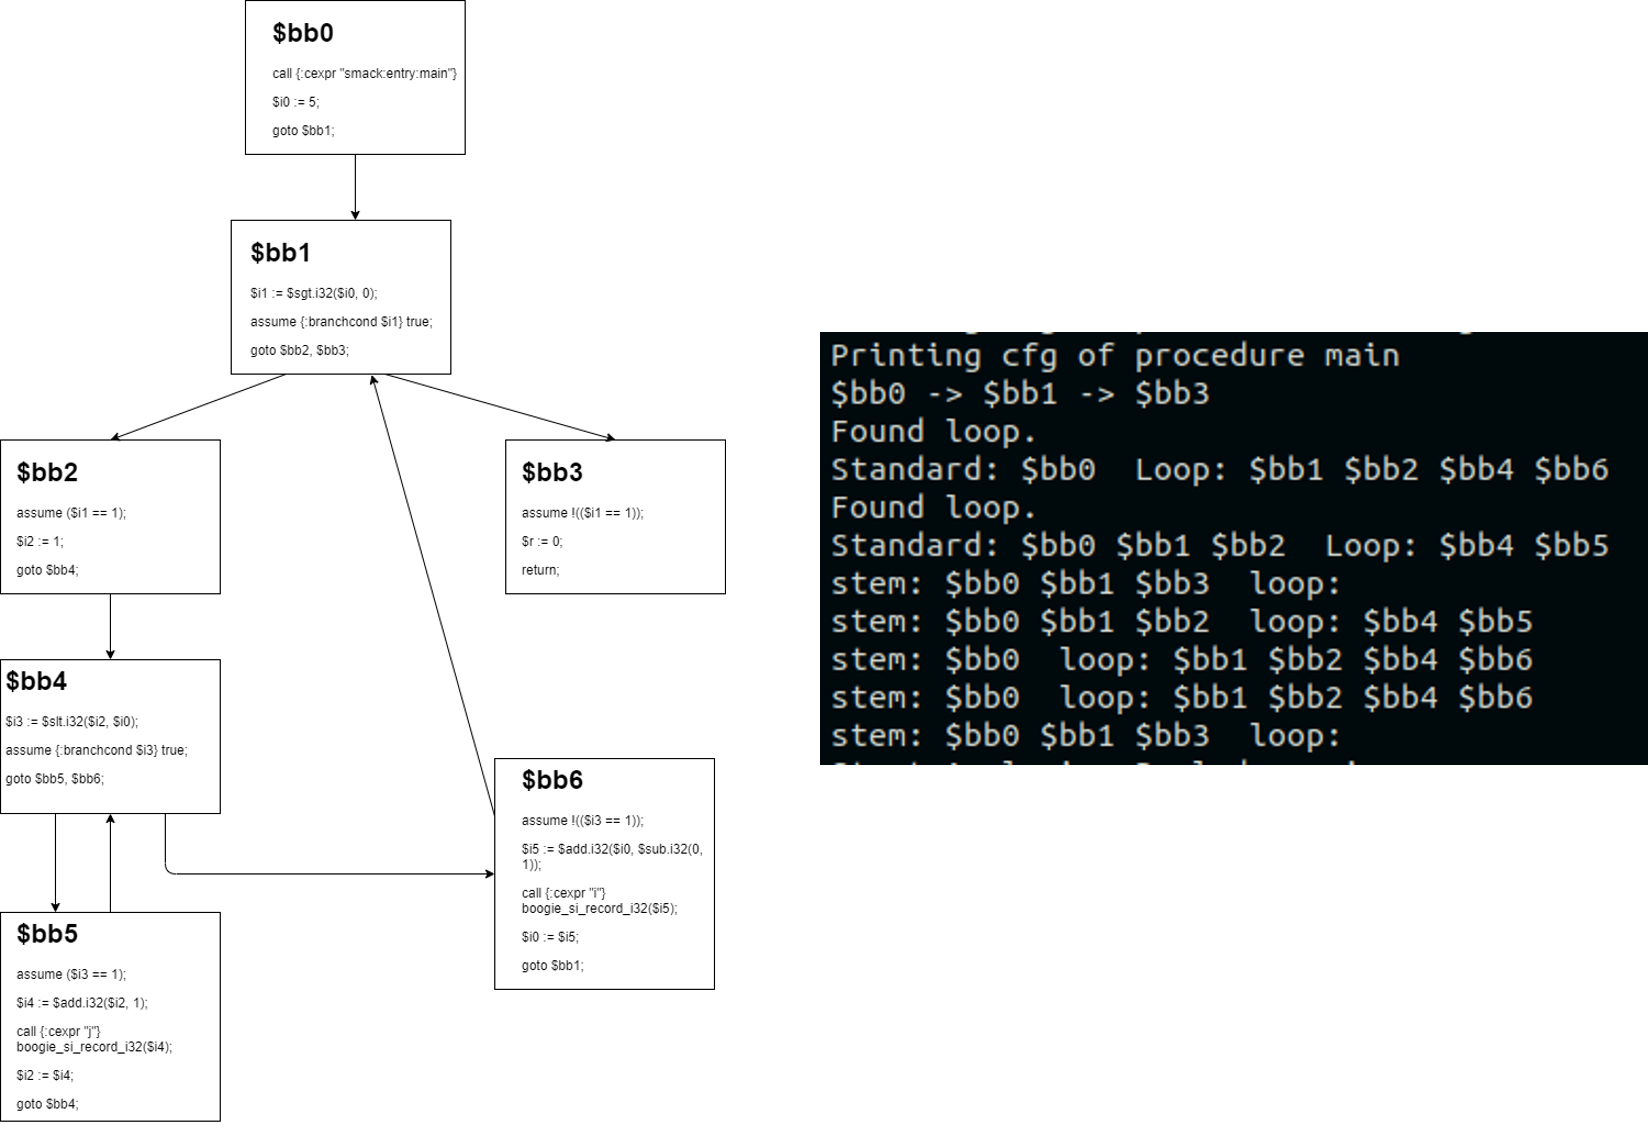
\includegraphics[width=0.7\linewidth]{lasso.jpg}
\end{figure}
\end{itemize}    
\end{frame}

\begin{frame}{冯维直:Plan}
    
    \begin{itemize}
        \item 本周主要工作计划:将Lasso Ranker和SVM Ranker集成到工具中,使其能判断sample得到的一条lasso的终止性。
\end{itemize}    
\end{frame}

\begin{frame}\frametitle{Differential Privacy}
Currently:
\begin{itemize}
  \item APLAS extension: complete the ePMC plugin, writing the tool description now;
\end{itemize}

Plan:
\begin{itemize}
  \item Finish the description and polish the article(including Abstract, Introduction...);
\end{itemize}

\begin{figure}[htbp]
    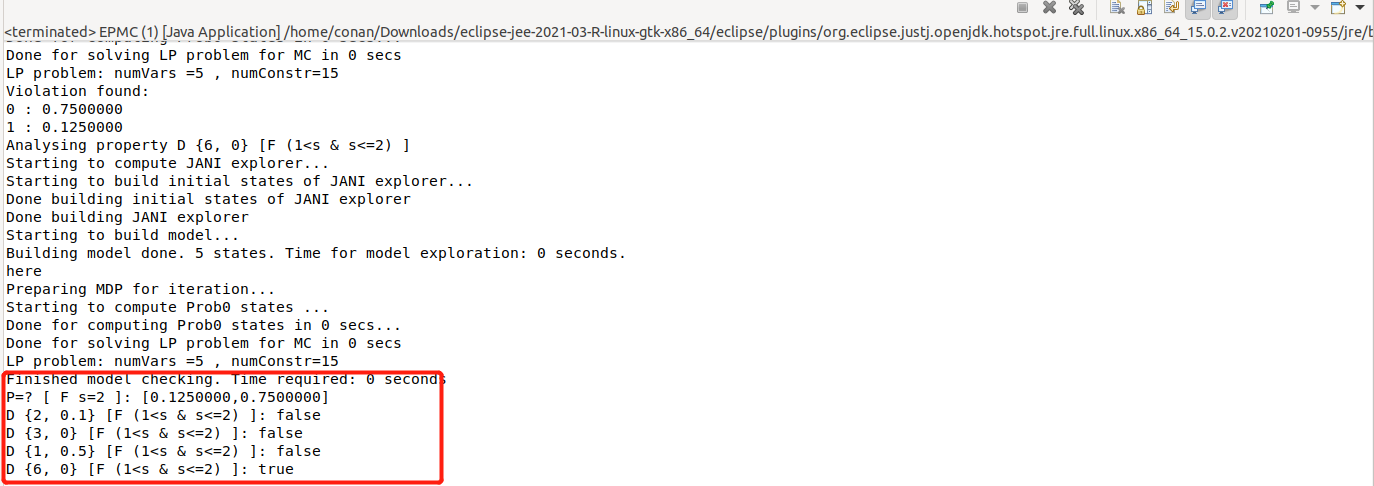
\includegraphics[width=1\linewidth]{epmc.jpeg}
\end{figure}
\end{frame}


\begin{frame}\frametitle{Pufferfish Privacy}
Currently:
\begin{itemize}
  \item Pufferfish: Learning to write scripts of Sagemath to compute integrals for continuous noise. (The limit is with only finite inputs/outputs.)
\end{itemize}

Plan:
\begin{itemize}
  \item Calculate more mechanisms..
\end{itemize}
\begin{figure}[htbp]
    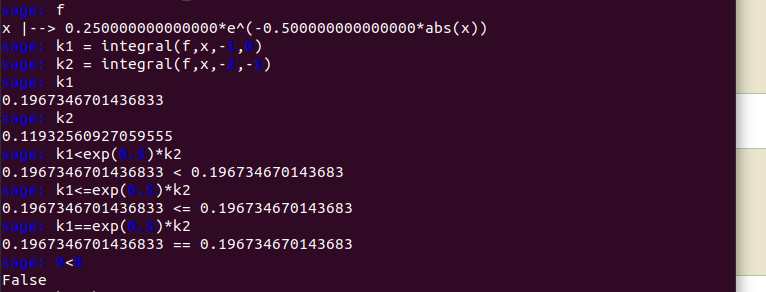
\includegraphics[width=0.8\linewidth]{saga.jpeg}
\end{figure}
\end{frame}
\end{document}